\chapter{The thermal conductivity of strained graphene\label{chap:therm}}
If the out of plane acoustic (ZA) phonons in graphene were a person, they might be characterized as productive egomaniacs.
They are believed to enable graphene's very high thermal conductivity by contributing more than 70\% of the thermal conductivity of suspended graphene \cite{Lindsay2010}.
These same phonons are thought to suppress the potentially divergent thermal conductivity contributions from the in plane acoustic phonons \cite{Pereira2013,Bonini2012}.
Both of these conflicting contributions are linked to the atypical quadratic dispersion of the ZA phonons.
Using strain and pressure we modify the ZA phonons while measuring the thermal conductivity.
This should help isolate the importance of the ZA phonnos and further test our understanding of graphene's high thermal conductivity.

\section{Experimental background \label{sec:therm:Exp}}
Balandin and coworkers were the first to measure the thermal conductivity of gra\-phene.
They reported that suspended graphene had a record high thermal conducitivity of roughly 5000 W/m-K \cite{Balandin2008}.
Shortly thereafter measurements of supported graphene showed a more modest thermal conductivity of roughly one six of the original \cite{Seol2010}.
This discrepancy has been the source of heavy study in the years since.

The original measurements were performed on suspended graphene samples using an optical technique.
This creative technique uses a laser excitation to heat the sample and the temperature induced energy shift of the Raman scattered light to measure temperature; the Raman measurement provides both a heat source and a thermometer.
When used in conjunction with a heat transfer model, this is enough to determine the thermal conductivity.
This technique has advantages and disadvantages.
The required samples are very simple to fabricate and the measurement is fairly standard.
However, the measured thermal conductivity depends on a variety of parameters that are hard to measure including the optical absorption of the graphene, the laser spot size, and the temperature dependence of the phonon modes.
What's more, the results depend on the accuracy of the thermal transport model which inherently cannot account for ballistic thermal transport.
Nonetheless, the simplicity of this technique has resulted in a variety of publications studying aspects of thermal transport in suspended graphene \cite{Balandin2008,Faugeras2010,Cai2010,Ghosh2010,Lee2011,Chen2011a,Chen2012}.

The Raman measurement technique has since been advanced in a series of publications.
Faugeras \textit{et al.} was first to study graphene suspended over a circular aperture.
This circular symmetry of this geometry simplifies the heat transfer model.
Additionally, they used the Raman Stokes to anti-Stokes ratio as an independent temperature measurement validating the use of phonon energy shifts to measure temperature \cite{Faugeras2010}.
Cai \textit{et al.} advanced the thermal transport model by including the thermal transport to the substrate instead of treating supported graphene as a heat sync.
Chen \textit{et al.} further advanced the thermal transport model to include thermal conductivity to the surrounding gas \cite{Chen2011a}.

The measurement which yielded the more modest values of thermal conductivity were direct measurements of supported graphene.
In these more traditional measurements resistive heaters are used to create a temperature gradient and solid state thermometers are used to measure the temperature.
The thermal conductivity of graphene is then determined directly from the thermal resistance of the graphene.
Although certainly less error prone, there has been only one other measurement of the thermal conductivity of graphene using this technique \cite{Jang2010}.
This is a result of the more difficult measurement and much more difficult sample fabrication.

Figure \ref{fig:therm:lit} summarizes all of the reported room temperature thermal conductivity measurements of single layer graphene.
The thermal conductivity decrease from a value of roughly 2000 W/m-K for suspended graphene, to a value close to 500 W/m-K for graphene supported on one side, to a value of less than 160 W/m-K for graphene encased in SiO$_2$ \cite{Jang2010}.
It is clear that graphene's thermal conductivity is negatively effected by the presence of a supporting or encasing bulk material.
The different thermal conductivities cannot be attributed to the different measurement techniques, a nanoscale thermal conductivity measurement also observed an increase in thermal conductivity for suspended few layer graphene \cite{Pumarol2012}.

\begin{figure}
	\begin{center}
	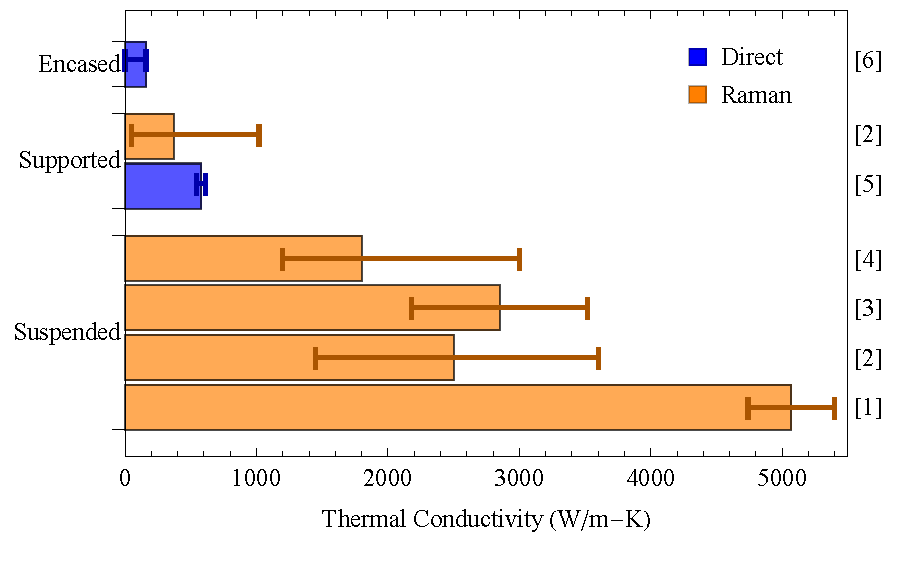
\includegraphics{Figs_Thermal/Thermal_lit.pdf}
	\end{center}
	\caption[Environmental dependence of graphene's thermal conductivity]{
	\label{fig:therm:lit}
		Summary of the reported values of the room temperature thermal conductivity of monolayer graphene grouped by the environment of the graphene: Suspended, supported on a bulk substrate, and encased in amorphous SiO$_2$.
		The color code indicates whether the measurements were performed using the Raman technique or a direct technique.
		The numbers on the right indicate the source: [1] is \cite{Balandin2008}, [2] is \cite{Cai2010}, [3] is \cite{Chen2011a}, [4] is \cite{Lee2011}, [5] is \cite{Seol2010}, [6] is \cite{Jang2010}.
		Error bars are taken from the literature.
	}
\end{figure}

\subsection{Theoretical background}
In response to the environmental dependence of the thermal conductivity, Lindsay and coworkers argued that the ZA phonons contribute more than 70\% of the very high thermal conductivity of suspended graphene \cite{Seol2010}.
This comes about for two reasons.
First, the quadratic dispersion gives a high density of states throughout the BZ.
Second, the in plane reflection symmetry provides a selection rule that limits the scattering phase space \cite{Lindsay2010}.
When the graphene is in contact with bulk materials the ZA phonons either leak into the surrounding media, are scattered by it, or are dampened by it, lowering the thermal conductivity.

The ZA phonons are also believed to limit the potentially divergent thermal conductivity contribution of the in plane phonons.
Klemens showed that the linear in plane acoustic phonons should contribute a logarithmically divergent thermal conductivity in graphene \cite{Klemens2001}.
This divergence follows from the frequency dependence of the terms which make up the thermal conductivity, $\kappa=\frac{1}{3} \int C v_G l(\omega) \rho(\omega) \ d\omega $, where $\kappa$ is the thermal conductivity, $C$ is the specific heat, $v_G$ is the group velocity of the acoustic phonons, $l(\omega)$ is the scattering length, and $\rho(\omega)$ is the density of states.
For a two dimensional phonon gas with linear dispersion $\rho(\omega) \propto \omega$ while for anharmonic scattering between linear acoustic phonons $l(\omega) \propto 1/\omega^2$.
Hence, in the absence of extrinsic scatterers, the integrand scales as $1/\omega$ and $\kappa$ diverges logarithmically.
The logarithmic divergence in $\omega$ should translate to a logarithmic divergence in device size \cite{Klemens2001}.
Larger devices should exhibit larger thermal conductivities because they support more of the long wavelength phonons that contribute strongly to the thermal conductivity.
To date this logarithmic divergence has not been observed \cite{Chen2011a}.

Pereira and coworkers believe that the ZA phonons suppress this divergence.
When these ZA phonons are neglected in equilibrium molecular dynamics the thermal conductivity diverges in agreement with Klemens, but when they are included the thermal conductivity converges to a large but finite value \cite{Pereira2013}.
It is believed that this is due to the ZA phonons near the center of the BZ.
With near zero group velocity these phonons cannot enhance thermal conductivity, but, with a large population, they can effectively scatter the in-plane phonons and eliminate the divergence.
Thus, the ZA phonons are the main contributor to graphene's thermal conductivity only because the low energy ZA phonons suppress the divergent thermal conductivity of the in plane phonons.

Simulations by both Pereira \cite{Pereira2013} and coworkers and Bonini and coworkers \cite{Bonini2012} show that strain could act to liberate the divergent thermal conductivity contribution of the in plane phonons.
By linearizing the ZA phonon modes near the $\Gamma$ point, strain decreases the density of states of the zero group velocity ZA phonons which scatter with the in plane phonons.
Uniaxial strain of 2 \% should reduce this scattering enough to realize the divergent thermal conductivity of the in plane phonons \cite{Pereira2013} while for biaxial strain any amount of strain should be enough \cite{Bonini2012}.

\section{Tuning the ZA phonon}
Although the theory discussed to this point is convincing, it deserves further testing.
It was built around only two data points: The high thermal conductivity of suspended graphene and the lower thermal conductivity of supported graphene.
Further, the resulting theory relies on the exotic, quadratically dispersed, ZA phonons which have only been measured directly in graphene mechanical resonators.
The thermal transport can be more deeply understood by altering the ZA phonon and measuring the change in thermal conductivity.

The ZA phonons can be continuously tuned while the thermal conductivity is measured \textit{in situ} using the device geometry from Chapter \ref{chap:fri}.
The phonons are altered in two ways.
First, the strain induced in pressurized graphene sealed microchambers linearizes the ZA phonon dispersion.
As discussed in the previous section, this might increase the thermal conductivity by liberating the divergent thermal conductivity of the in plane phonons \cite{Pereira2013,Bonini2012}.
Second, the gas surrounding the suspended graphene should lower the lifetime of the ZA phonons.
This has been observed in graphene mechanical resonators which exhibit decreased quality factors in ambient pressure compared to vacuum \cite{Bunch2007}.
Lowering the phonon lifetime should lower their contribution to the thermal conductivity.
Tuning the ZA phonon in these ways and measuring thermal conductivity should provide deeper insight into the mechanism behind the high thermal conductivity of suspended graphene.

\subsection{Measurement}
The experimental geometry described in Section \ref{sec:fri:Exp} enables the thermal conductivity to be measured while the ZA phonons are tuned.
The phonons are tuned by setting the external pressure, $P$, to gauge pressures which range from -0.1 MPa of vacuum to 0.69 MPa of overpressure.
Measuring with the external pressure both greater than and less than the internal pressure $P_0$ enables us to decouple strain and pressure effects.
Pressure effects should increase monotonically with pressure while strain effects should initially lesson as $P$ approaches $P_0$ and the graphene flattens out but then increase when $P$ surpasses $P_0$.

The Raman technique described in Section \ref{sec:therm:Exp} is used to measure the thermal conductivity.
Linearly polarized, 514.5 nm laser light from an Argon Ion laser is focused on the center of the microchamber.
The focused beam waist, measured the same way as in Section \ref{sec:fri:Raman}, is $0.66 \pm 0.04$ nm.
The power which reaches the sample is tuned by changing the laser power and not by changing ND filters.
This ensures that the centering of the beam is not power dependent.
The power which reaches the sample is calculated from the power measured at the exit port of the Renishaw using the system throughput of $0.67 \pm 0.01$.
The laser stability over the measurement period is 2 \%.

The temperature is measured using the heating induced shifts of the measured G and 2D energies $\Delta \omega=\chi \Delta T$, where $\Delta T$ is the change in temperature and $\chi$ represents the temperature dependence of the phonon energy arising due to anharmonicities \cite{Bonini2007}.
As starting points we use the values measured by Chen \textit{et al.} on suspended CVD graphene: $\chi_G=-(4.4 \pm 0.3) \times 10^{-2} \ cm^{-1}/K$, $\chi_{2D}=-(7.2 \pm 0.2) \times 10^{-2} \ cm^{-1}/K$ \cite{Chen2011a}.
Other measurements report lower values \cite{Calizo2007}, and hence, higher thermal conductivities \cite{Balandin2008}, but these values were measured on supported graphene where the different thermal expansion coefficients of graphene and the substrate could be more of an issue.
Since these temperature related shifts happen because of phonon anharmonicities, they may have some strain dependence.
The Anti-Stokes to Stokes ratio could be used as an alternative, anharmonicicty independent temperature measurement.
However, we found that these measurements were not useful; they took too long and were too hard to interpret.

The temperature can be calculated from the frequency shift which results from raising the power from $P_{lo}$ to $P_{hi}$ 
Assuming that the thermal resistance, $R=\frac{\Delta T}{P}$ where P is the absorbed power, is constant gives
\begin{equation}
	T_M=T_{hi}-T_0=\frac{\Delta \omega}{\chi} \frac{P_{hi}}{P_{hi}-P_{lo}} \ , \label{eq:therm:TM}
\end{equation}
where $T_0$ is ambient temperature and $T_M$ is referred to as the measured temperature.
The corresponding measured thermal resistance is $T_M/P_{hi}$.
These values are referred to as measured temperatures because they represent a weighted average over the finite spot of the laser beam.

The heat transfer model described in Appendix \ref{chap:HTM} is used to extract the thermal parameters from the measured temperature.
The model depends on the thermal conductivities of the suspended graphene, $\kappa_{SS}$, and the supported graphene, $\kappa_{SP}=(579 \pm 34) \ W/m-K$ \cite{Seol2010}, as well as the interface thermal conductivities to the gas, $g_G$, and to the substrate $g_S=(50 \pm 13) \ MW/m^2-K$ \cite{Mak2010}.
An example temperature distribution predicted by this model is shown in figure \ref{fig:therm:HTPlot}.
As one might expect, the temperature rise is the greatest where the laser is heating, near the center of the microchamber.
At the edge of the microchamber the slope is discontinuous due to the change in thermal conductivity.
Where the thermal conductivity is lower it takes a larger temperature gradient to conduct the same heat energy.
The green shaded region represents the radial envelope of the excitation profile.
It illustrates that $T_M$ is not the temperature rise at the center of the hole but is rather an average over a radial window.
Appendix \ref{chap:HTM} describes how $T_M$ can be used to find the thermal parameters.

\begin{figure}
	\begin{center}
	\begin{tikzpicture}[scale=1]

	%The temperature profile
	\node at (0,0) {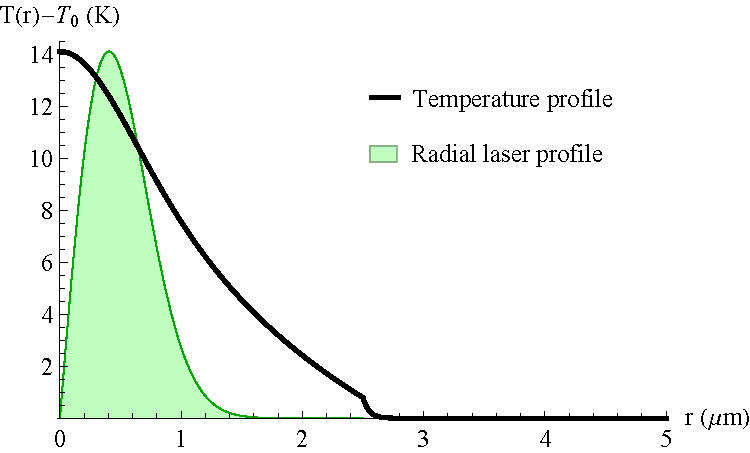
\includegraphics{Figs_Thermal/TemperatureProfile.pdf}};
	
	%The Differential Equations
	\node at (-2.8,-2.25) [fill=white, opacity=.75, text opacity=1,rounded corners=6 pt,inner sep=1.5 pt] {$\kappa_{SS} \nabla^2 T(r) + \dot{Q_L} - \dot{Q_g} =0$};
	\node at (3,-2.25) {$\kappa_{SP} \nabla^2 T(r) - \dot{Q_S} - \dot{Q_g} =0$};
\end{tikzpicture}
	\end{center}
	\caption[Expected temperature distribution in a graphene sealed microchamber heated by a centered laser]
	{\label{fig:therm:HTPlot}
		Theoretical temperature distribution in a graphene sealed microchamber heated by a centered laser.
		The black curve shows the temperature increase for a 5 $\mu$m diameter microchamber assuming that $\kappa_{SS}=2000 \ W/m-K$ and  $g_{G}=0.03 \ MW/m^2-K$ \cite{Chen2011a}.
		The radial profile of the 1.5 mW laser heat source with a 0.81 $\mu$m waste is overlaid in green.
	}
\end{figure}

The samples described in Table \ref{tab:therm:samples} were measured by taking Raman spectra with multiple excitation powers across a range of pressures.
The number of layers was found using Raman spectroscopy and optical interference, the radius and hole depths were measured using low force contact mode AFM, and the maximum strain was calculated using Hencky's model \cite{Hencky1915}.
Device fabrication was either done using the standard mechanical exfoliation technique or by using a polymer based align transfer technique \cite{Goossens2013T}.
Pressures were decreased in increments from 0.69 MPa to -0.1 MPa and then increased back to 0.69 in interspaced increments to monitor for any hysteretic response.
These measurements allowed for the extraction of the pressure dependent measured thermal resistance.

\begin{table}
	\begin{center}
	\begin{tabular}{l c c c c c c}
		\hline
		\hline
		Samples & NL 	& Radius 					& Depth 		& $\epsilon_{max}$ & Fabrication 		& Sealed? \\
		\hline
		FFF		& 1 	& $(3.09 \pm 0.04)$ $\mu$m 	& $>$ 5 $\mu$m 	& 1.2 \%	& Transferred 	 	& no \\
		SB07-1	& 1 	& $(2.74 \pm 0.08)$ $\mu$m 	& $\simeq$ 230 nm & 1.1 \%	& Exfoliated 		& yes \\
		SB08-2	& 2 	& $(1.52 \pm 0.07)$ $\mu$m 	& $>$ 3 $\mu$m 	& 0.46 \%	& Exfoliated 		& yes \\
		SB03-2	& 3 	& $(4.99 \pm 0.01)$ $\mu$m 	& $>$ 5 $\mu$m 	& 0.77 \%	& Exfoliated 		& yes \\
		\hline
		\hline
	\end{tabular}
	\end{center}
	\caption[Samples used in thermal conductivity measurements]{\label{tab:therm:samples} 
	Details of the samples used in thermal conductivity measurements. NL refers to the number of layers and $\epsilon_{max}$ is the maximum strain.}
\end{table}

\subsection{Data analysis}
Peak positions were found by fitting the measured spectra to representative spectral shapes.
The G peak was fit to a single Lorentzian for all four samples.
The best fit to the 2D peak depends on the number of layers.
For monolayer, suspended graphene the 2D peak is best fit by two Lorentzians with equal widths separated by 14 wavenumbers \cite{Berciaud2013}.
To limit the number of fitting parameters, the ratio of the peak amplitudes was taken as the average of the best fits: 3.44.
For bilayer graphene the 2D peak is best fit by 4 Lorentzians with equal widths \cite{Ferrari2006,Malard2007}.
The fitting parameters were restricted to an amplitude, a width, and a position by setting the separation between peaks and the relative amplitudes between peaks based on the average best fits.
An example of the best fit to a bilayer spectra is shown in Figure \ref{fig:therm:spec}
Since there is no well excepted form for the trilayer 2D band, the temperatures were only determined from the G band data for sample SB03-2.

\begin{figure}
	\begin{center}
	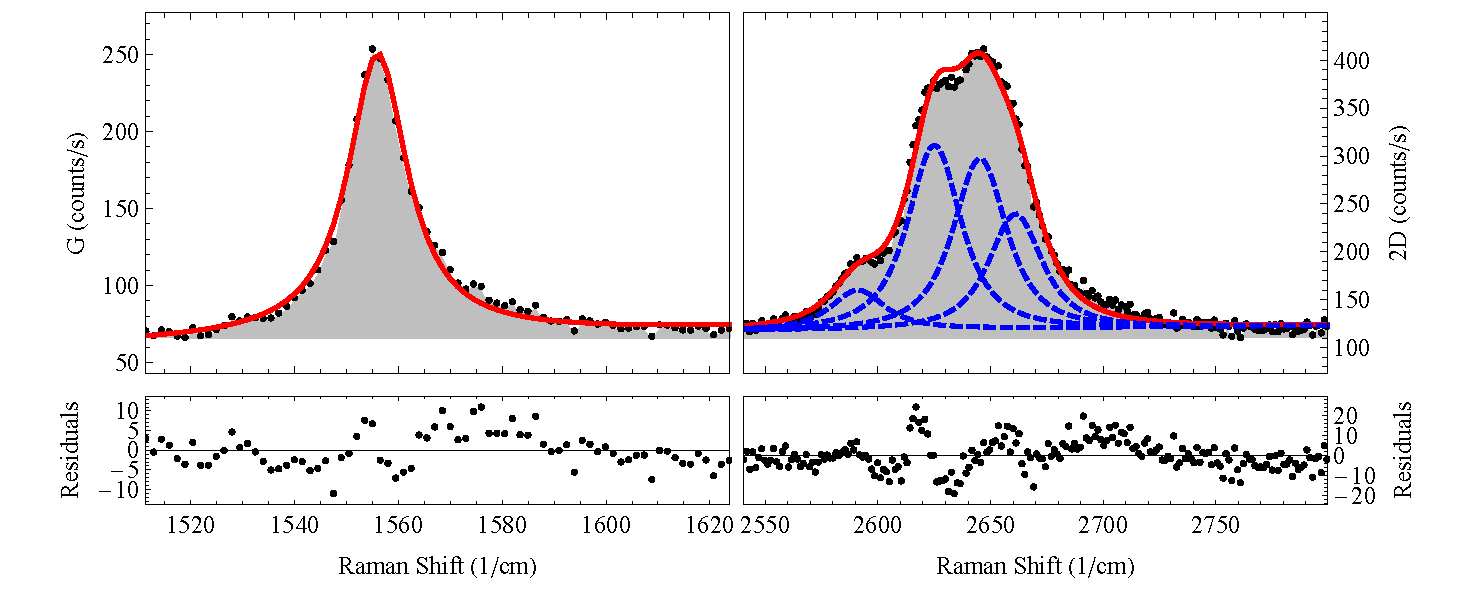
\includegraphics[scale=0.6]{Figs_Thermal/0_3mW.pdf}
	\end{center}
	\caption[Representative fit to Raman spectra for thermal conductivity measurements]{\label{fig:therm:spec}
		A representative best fit to the Raman spectra taken at the center of bilayer sample SB08-2 using 2 mW of incident power at 0.69 MPa of gauge pressure.
		The restricted four Lorentzian fit to the 2D spectra matches the data well.
	}
\end{figure}

Figure \ref{fig:therm:PeakPressure} shows the best fit positions of the G and 2D bands as a function of pressure for bilayer sample SB08-2.
As discussed in detail in Chapter \ref{chap:fri}, the Raman bands depend linearly on strain which in turn scales as $(P-P_0)^{2/3}$.
This describes the overarching trend in the pressure response and can be used to determine $P_0$.
The data in the figure is fit by the expected pressure dependence and the extracted value of $P_0$ is indicated by the black vertical line.
The effects of laser heating is hidden in the fine structure.
As laser heating increases, the peaks slightly red shift as shown by the systematically lower peak positions measured with the higher excitation powers.
Samples SB07-1, SB08-2, and SB03-2 exhibit this type of pressure dependent response, FFF, on the other hand, exhibits no pressure response indicating that the membrane is leaky.
This leaky sample is useful as it decouples the pressure and strain response.

\begin{figure}
	\begin{center}
	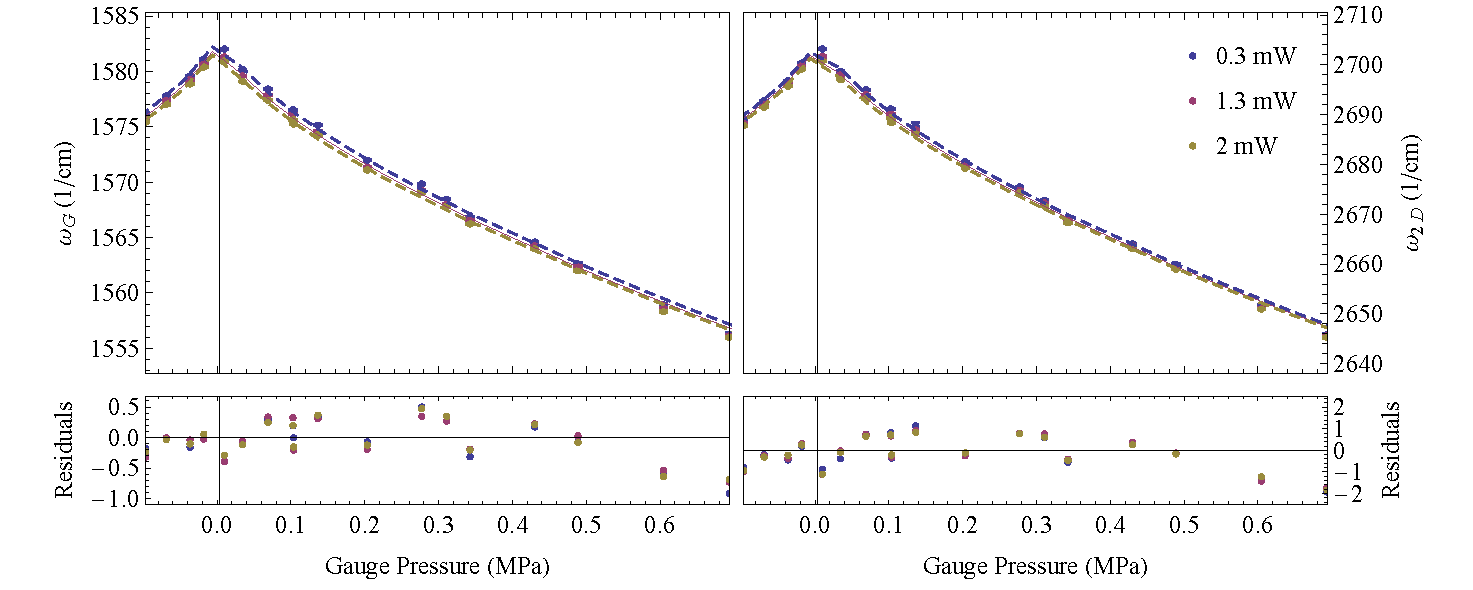
\includegraphics[scale=0.6]{Figs_Thermal/PeakPressure.pdf}
	\end{center}
	\caption[Pressure dependent peak positions]{\label{fig:therm:PeakPressure}
		The peak positions measured as a function of applied pressure using three different laser excitation powers for bilayer sample SB08-2.
		The peak positions are fit to the expected $(P-P_0)^{2/3}$ behavior and the best fit value for $P_0$ is indicated by the black vertical line.
		Increasing laser excitation power downshifts the peaks.
	}
\end{figure}

The calculation of $T_M$ using Equation \ref{eq:therm:TM} is complicated by optical interference.
In sample SB07-1 the measured temperatures exhibit an oscillatory behavior in pressure.
As shown in Figure \ref{fig:therm:Inter}, these oscillations are correlated with similar oscillations in the measured G and 2D areas.
This suggests that the observed behavior is driven by optical interference in the excitation beam.
As overpressure is applied to the graphene it is pushed into the microchamber moving it from a point where the excitation undergoes destructive interference, to a point of constructive interference, and then back to a point of destructive interference.
As the interference changes, the amount of power heating the graphene changes, and thus, so does the temperature.
The interference interpretation is supported by the agreement between the number of interference minimum and the expected displacement at the center of the graphene.
Minimum are expected every half wavelength and from -0.1 MPa to 0.69 MPa the graphene displaces by 508 nm or roughly one wavelength consistent with the two minimum in Figure \ref{fig:therm:Inter}.
The interference in SB07-1 is the strongest, but all of the other devices exhibit similar interference phenomena.
The Rayleigh range of the focused beam is $\sim 2.7$ $\mu$m indicating that even microchambers with depths of 8 $\mu$m might be expected to exhibit weak interference effect.
Interestingly, even leaky sample FFF shows very slight signs of interference.
This is probably due to the nonlinearity of the pressure deflection curve.
In the low pressure regime small pressure changes cause relatively large deflections; for FFF a differential pressure of 0.001 MPa would cause a deflection of 40 nm.

\begin{figure}
	\begin{center}
	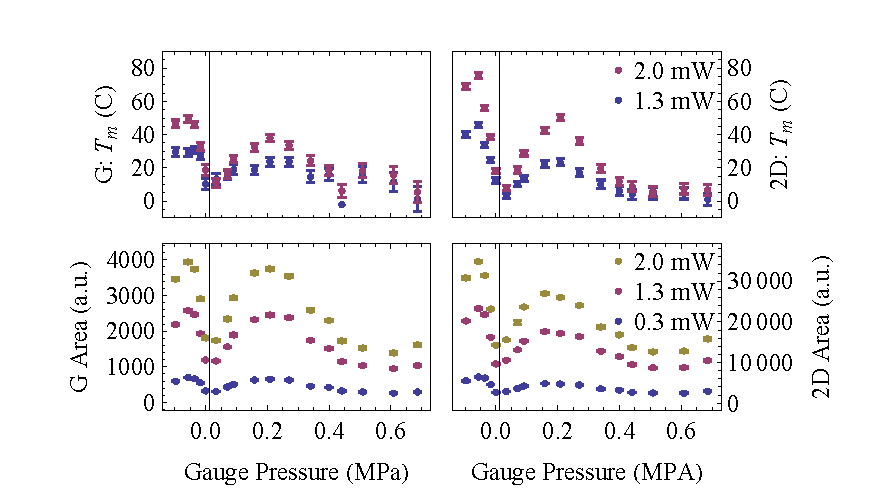
\includegraphics{Figs_Thermal/inter.pdf}
	\end{center}
	\caption[Issues with optical interference in thermal conductivity measurements]{\label{fig:therm:Inter}
		A comparison of the temperatures calculated from the shifts of the G peak (top, left) and the shifts of the 2D peak (top, right) with the measured areas of the G peak (bottom, left) and 2D peak (bottom, right).
		Measurements were taken on monolayer sealed sample SB07-1.
		The oscillatory behavior in all four plots suggests that the observed behavior is a result of optical interference.
	}
\end{figure}

The optical interference of the excitation beam can be estimated from the oscillatory behavior of the Raman signal.
The oscillations in the Raman signal are driven by the product of the optical interference of both the incident beam and the outgoing beam.
Treating the system as a plane wave incident on a perfect mirror, the product of these two terms is $4 \sin^2(k z) \sin^2(k_R z)$ where $z$ is the distance of the graphene above the mirror, $k$ is the spatial frequency of the laser excitation, and $k_R$ is the spatial frequency of the inelastically scattered light.
A more rigorous calculations using transfer matrices and optical constants from Palik \cite{Palik1991} shows the expected behavior with a negligible 2 \% constant offset that originates because silicon is not a perfect mirror.
The oscillations in the measured temperature, however, are only due to the interference in the incident beam: the $2 \sin^2(k z)$ component.
The fact that the exact depths of the microchambers are not known and the interference we observe in the interference in a Gaussian beam, a direct calculation of the incident power from the oscillations in the Raman areas is not possible.
Instead, we approximate $4 \sin^2(k z) \sin^2(k_R z) \simeq 4 \sin^2(k z) = (int(z))^2$.
This allows an estimation of the interference in the excitation beam.

The observed oscillations in the G and 2D areas are on top of a constant offset.
The constant offset is believed to be signal not driven by interference.
Thus, the interference function is calculated as
\begin{equation*}
	Area=P_i \ A+P_i \ B\ int(z)^2/4 \rightarrow  int(z)=2\sqrt{\frac{Area/P_i-A}{B}}
\end{equation*}
where $P_i$ is the power of the incident beam, and $A$ and $A+B$ are the minimum and the maximum of the $P_i$ normalized areas, respectively.
The intensity of the incident beam at the sample is then given by $P_i(A+ B \ int(z))$

Also--redo the corrected spectra

The pressure dependence of the measured thermal resistance is measured in several different ways.
For samples FFF, SB07-1, and SB08-2 both the G and 2D shifts can be used to calculate $R_M$.
The values of $\chi$ reported by Chen \textit{et al.} \cite{Chen2011a} provided good agreement between G and 2D data for samples SB07-1 and SB08-2.
However, for sample FFF a slight offset was required to achieve good agreement.
The values of $\chi$ for the G and 2D peaks needed to be increased and decreased by $0.6 \times 10^{-2}$ respectively.
Samples SB07-1, SB08-2, and SB03-2 were measured at three different powers providing two additional measurements of $R_M$.
Averaging all of the redundant measurements gives smaller uncertainties.
Figure \ref{fig:therm:R_average} shows an example of the averaged $R_M$ data.
The individual $R_M$ measurements are in good agreement justifying the averaging.

\begin{figure}
	\begin{center}
	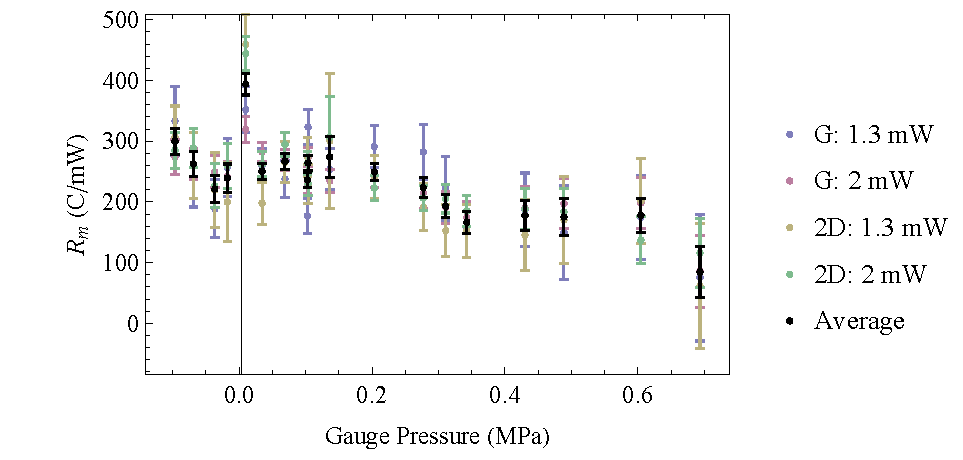
\includegraphics[scale=0.8]{Figs_Thermal/R_average.pdf}
	\end{center}
	\caption[Average pressure dependence of the measured thermal resistance]{\label{fig:therm:R_average}
		The average measured thermal resistance corrected for interference of bilayer sample SB03-2.
		The four different measurements used to calculate the average are in good agreement.
		The black vertical line is positioned at $P_0$.
	}
\end{figure}

\subsection{Measured thermal resistances}
Plots as a function of pressure and strain

\subsection{Extracted thermal properties}
Description of thermal model

Method to extract parameters

\subsection{Conclusions}
How to eliminate optical interference